\documentclass[journal]{IEEEtran}

\usepackage{amsmath,amssymb}
\usepackage{booktabs}
\usepackage{multirow}
\usepackage{graphicx}
\usepackage{xcolor}
\usepackage{cite}
\usepackage{url}
\usepackage[hidelinks]{hyperref}
\usepackage{tikz}
\usetikzlibrary{arrows.meta,positioning}
\newcommand{\SourceDisjointGroups}{15}
\newcommand{\SourceDisjointClips}{190}
\newcommand{\SourceDisjointFraction}{18.38\%}
\newcommand{\OverlappingSourceGroups}{127}


\newcommand{\method}{\textsc{Amac}}
\newcommand{\todoauthor}{Author Name}
\newcommand{\todoaffiliation}{Affiliation to be supplied before submission}

\title{\method: Risk-Aware Commitment under Asynchronous Modality Arrival for Multimodal Affective Agents}

\author{\todoauthor%
\thanks{\todoaffiliation. Corresponding email and ORCID must be supplied before submission.}}

\begin{document}

\maketitle

\begin{abstract}
Multimodal affect recognition is usually evaluated after text, audio, and vision are all available, but an interactive agent may receive these modalities at different times. A provisional affect state can therefore be useful before complete evidence arrives, yet an incorrect early state can trigger an unsuitable response and a later state change can make the agent inconsistent. We formulate this problem as asynchronous affect commitment and introduce the Anytime Multimodal Affect Contract (\method), which estimates whether the state inferred from the currently visible modality prefix is correct and maps that estimate to \textsc{wait}, \textsc{commit}, or \textsc{revise}. The terminal state is forced to equal the prediction from all three modalities, separating commitment quality from final recognition accuracy. On the official CH-SIMS v2 test split, evaluated under all six modality orders, the risk estimator fixed in the archived local protocol before sealed-test evaluation reduces preterminal committed error by 12.14 percentage points and revisions by 11.67 points relative to a grid-selected fixed-confidence policy at approximately 91\% stage-two coverage; post-hoc source-video-group bootstrap intervals preserve both directions. A method-locked diagnostic compares logistic risk estimation with Platt and isotonic calibration across a common risk--coverage interval; it is interpreted as evidence about the tested feature sets rather than a formal non-inferiority or universal calibration result. An EmotionTalk contract-level evaluation is consistent with error reduction, but not revision reduction, in three held-out groups. A stateful Go agent tool exactly reproduces 18,612 frozen offline decisions. These results support risk-aware commitment as a measurable layer between multimodal perception and affect-conditioned agent action, while overlapping source groups in the official split limit claims of cross-source generalization.
\end{abstract}

\begin{IEEEkeywords}
affective computing, multimodal sentiment analysis, intelligent agents, selective prediction, asynchronous modalities, uncertainty estimation
\end{IEEEkeywords}

\section{Introduction}

\IEEEPARstart{M}{ultimodal} affective agents use words, prosody, and facial behavior to estimate a user's state. Modern multimodal sentiment and emotion models improve representation and fusion when all streams are available \cite{tsai2019mult,hazarika2020misa,yu2021selfmm}. Interactive systems face an additional decision that conventional benchmark accuracy does not measure. The agent must decide whether its current estimate is reliable enough to affect a response while some modalities are delayed, missing, or still being processed.

This timing decision matters even when the final multimodal predictor is fixed. A text prefix can appear neutral while vocal tone indicates distress, or a visual cue can overturn an early positive interpretation. An agent that immediately acts on each provisional state exposes users to errors and may change its behavior repeatedly. An agent that always waits for all inputs avoids early errors but forfeits responsiveness. The operational question is therefore not only which affect state is eventually predicted, but when a provisional state becomes actionable and when an earlier commitment should be revised.

Existing research addresses adjacent parts of this problem. Missing-modality methods learn representations that remain accurate when a stream is absent \cite{lin2023missmodal,li2024umdf,huang2026recap,miyoshi2026dqf}. Selective prediction permits a classifier to abstain at a chosen coverage \cite{geifman2019selectivenet}, while early-exit methods balance computation and accuracy across network depth \cite{zhou2020pabee,jazbec2023anytime,jazbec2024risk}. Affective-agent toolkits and recent multi-agent emotion systems integrate multimodal perception into dialogue or reasoning \cite{li2020adviser,wang2026affectagent}. These formulations do not directly measure the sequence of affect states that becomes visible as heterogeneous modalities arrive, including the cost of exposing a wrong state and revising a previous commitment.

We study this gap with an author-defined protocol built on public multimodal datasets. Each clip is expanded into the six permutations of text (T), audio (A), and vision (V). At each prefix, a frozen upstream predictor produces a provisional affect state. \method{} estimates the probability that this state matches the labeled state and applies a stateful commitment contract. The contract can wait, make a first commitment, or revise a prior commitment. The third modality always forces the complete TAV state, which prevents the contract from improving or degrading terminal recognition by construction.

The study asks four questions. First, can learned current-prefix risk reduce committed error and revision at matched early coverage relative to fixed-confidence policies? Second, is any gain explained by ordinary scalar confidence calibration or a particular neural architecture? Third, does the effect transfer to a dataset with independent modality annotations? Fourth, does the implemented agent tool reproduce the offline contract under complete replay and invalid-input checks?

The paper contributes the following evidence. We formalize asynchronous affect commitment with explicit state transitions and metrics that separate early exposure, revision, coverage, and terminal identity. We evaluate every modality order while retaining official labels and data partitions where applicable. A one-shot CH-SIMS v2 official-split test supports lower error and revision than matched-coverage confidence policies, and a post-hoc source-group analysis quantifies the dependence limitation. Competitive diagnostics reject architecture-specific novelty and indicate that current-prefix features contain information beyond scalar calibration. An external EmotionTalk evaluation preserves the error direction while rejecting universal revision reduction. Finally, a stateful agent tool reproduces all frozen offline trajectories. The contribution is the commitment layer and its evaluation, not a new multimodal recognition backbone.

\section{Related Work}

\subsection{Multimodal Affect Recognition}

Multimodal sentiment analysis combines linguistic content with acoustic and visual behavior. MulT models cross-modal interactions without requiring explicit temporal alignment \cite{tsai2019mult}; MISA separates modality-invariant and modality-specific representations \cite{hazarika2020misa}; and Self-MM uses self-supervised auxiliary tasks to learn modality-specific representations \cite{yu2021selfmm}. CH-SIMS introduced Chinese clips with both multimodal and independent unimodal annotations \cite{yu2020chsims}. CH-SIMS v2 expanded this resource and emphasized the contribution of nonverbal cues \cite{liu2022chsimsv2}. These datasets make prefix-level analysis possible because T, A, and V predictions can be constructed for the same labeled clip.

Most benchmark protocols evaluate a fixed set of available modalities. Work on uncertain missing modalities instead asks a predictor to remain accurate when one or more streams are unavailable. MissModal aligns complete and incomplete representations without changing fusion \cite{lin2023missmodal}. UMDF uses self-distillation across uncertain missing patterns \cite{li2024umdf}, while more recent systems reconstruct coherent affective patterns or learn query-based fusion from incomplete inputs \cite{huang2026recap,miyoshi2026dqf}. These methods improve the prediction made from a given subset. Our setting holds the upstream subset predictors fixed and asks whether an agent should expose their outputs as modalities arrive. The two directions are complementary: a stronger missing-modality model can serve as the upstream predictor for the same commitment contract.

\subsection{Selective Prediction, Calibration, and Anytime Inference}

Selective prediction associates prediction risk with coverage by allowing a model to reject uncertain cases. SelectiveNet learns prediction and rejection jointly \cite{geifman2019selectivenet}. Post-hoc confidence estimators provide an alternative when a deployed predictor cannot be retrained \cite{cattelan2024confidence}. Calibration methods such as Platt scaling and isotonic regression map model scores to empirical probabilities \cite{platt1999probabilistic,zadrozny2002transforming}; temperature-based calibration is also effective for modern neural networks \cite{guo2017calibration}.

Anytime and early-exit models produce intermediate predictions before completing all computation. Patience-based exits use agreement among internal classifiers \cite{zhou2020pabee}. Later work observes that instance-level quality need not improve monotonically across exits \cite{jazbec2023anytime} and applies risk control to the exit decision \cite{jazbec2024risk}. Modality arrival differs from network depth because each step changes the evidence type rather than adding another layer of the same computation. A later modality can reverse the inferred affect state, and an interactive agent must manage the already exposed state. \method{} consequently models both first commitment and revision instead of a single reject-or-exit event.

\subsection{Affective Agents}

Multimodal conversational-agent platforms have incorporated emotion recognition, engagement prediction, and nonverbal signals into modular dialogue systems \cite{li2020adviser}. Recent work uses specialized agents and retrieval to improve final multimodal emotion recognition \cite{wang2026affectagent}. These systems motivate a clean interface between perception and action. \method{} supplies such an interface as a small state machine whose inputs are a provisional state and an externally estimated probability of correctness. It does not use an LLM's self-reported confidence, generate a dialogue response, or modify the perception model.

\section{Problem Formulation}

\subsection{Asynchronous Modality Prefixes}

Let a clip $i$ contain modalities $\mathcal{M}=\{T,A,V\}$ and a continuous sentiment label $y_i$. A modality order $\pi$ is one of the six permutations of $\mathcal{M}$. At stage $k\in\{1,2,3\}$, the visible subset is
\begin{equation}
S_{i,k}^{\pi}=\{\pi_1,\ldots,\pi_k\}.
\end{equation}
A frozen predictor $f_{S}$ maps the visible subset to a regression value $\hat{y}_{i,k}^{\pi}$. The discretization used in the contract is
\begin{equation}
q(u)=
\begin{cases}
-1, & u < -0.1,\\
0, & -0.1 \leq u \leq 0.1,\\
1, & u > 0.1.
\end{cases}
\end{equation}
The provisional state is $s_{i,k}^{\pi}=q(\hat{y}_{i,k}^{\pi})$, and the labeled state is $s_i^*=q(y_i)$. The regression output remains available for official terminal metrics, but the commitment contract operates on these three states.

The risk estimator receives only information visible at stage $k$. It predicts
\begin{equation}
r_{i,k}^{\pi}=P(s_{i,k}^{\pi}=s_i^*\mid z_{i,k}^{\pi}),
\end{equation}
where $z$ contains the current regression value, its absolute value, normalized arrival stage, a three-bit visible-modality mask, and a one-hot encoding of the current state. No future modality, label, dialogue response, or LLM confidence enters $z$.

\subsection{Commitment Contract}

The contract stores either no committed state, denoted $\varnothing$, or the most recently committed state $c_{i,k}^{\pi}$. Two parameters are frozen before evaluation: a first-commit threshold $\tau$ and a revision margin $\delta$. For $k<3$, the update is
\begin{equation}
c_k=
\begin{cases}
s_k, & c_{k-1}=\varnothing \land r_k\geq\tau,\\
s_k, & c_{k-1}\neq\varnothing \land s_k\neq c_{k-1}
       \land r_k\geq\tau+\delta,\\
c_{k-1}, & \text{otherwise}.
\end{cases}
\label{eq:contract}
\end{equation}
The externally visible action is \textsc{commit} for the first case, \textsc{revise} for the second case, and \textsc{wait} otherwise. At $k=3$, $c_3=s_3$ regardless of risk. This terminal rule isolates commitment behavior from the complete-modality predictor.

Figure~\ref{fig:overview} summarizes the interface. The risk estimator and contract sit between prefix perception and downstream affect-conditioned action. The contract can therefore be replaced, audited, or disabled without retraining the upstream predictor.

\begin{figure}[t]
\centering
\resizebox{\columnwidth}{!}{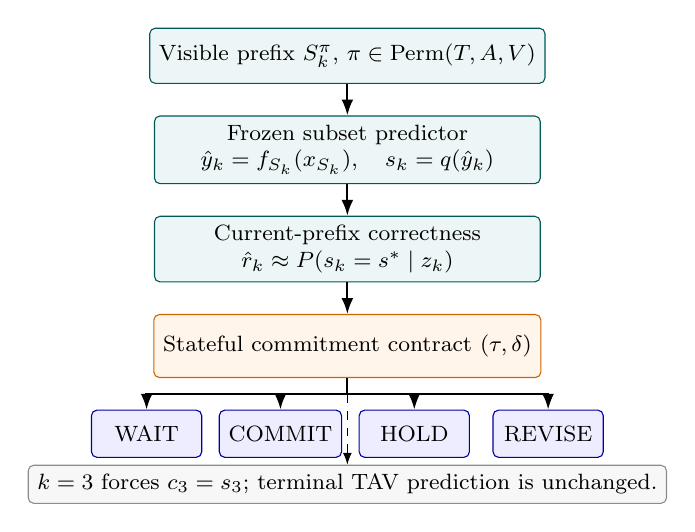
\begin{tikzpicture}[
  font=\footnotesize,
  node distance=4mm,
  block/.style={draw=teal!70!black, fill=teal!7, rounded corners=2pt, minimum height=7mm, minimum width=49mm, align=center},
  contract/.style={draw=orange!80!black, fill=orange!8, rounded corners=2pt, minimum height=8mm, minimum width=49mm, align=center},
  action/.style={draw=blue!65!black, fill=blue!7, rounded corners=2pt, minimum height=6mm, minimum width=14mm, align=center},
  note/.style={draw=black!45, fill=black!3, rounded corners=2pt, align=center},
  arrow/.style={-{Latex[length=2mm]}, thick}
]
\node[block] (arrival) {Visible prefix $S_k^\pi$, $\pi \in \mathrm{Perm}(T,A,V)$};
\node[block, below=of arrival] (predictor) {Frozen subset predictor\\$\hat y_k=f_{S_k}(x_{S_k}),\quad s_k=q(\hat y_k)$};
\node[block, below=of predictor] (correctness) {Current-prefix correctness\\$\hat r_k\approx P(s_k=s^*\mid z_k)$};
\node[contract, below=of correctness] (state) {Stateful commitment contract $(\tau,\delta)$};
\node[action, below=4mm of state.south, xshift=-25.5mm] (wait) {WAIT};
\node[action, below=4mm of state.south, xshift=-8.5mm] (commit) {COMMIT};
\node[action, below=4mm of state.south, xshift=8.5mm] (hold) {HOLD};
\node[action, below=4mm of state.south, xshift=25.5mm] (revise) {REVISE};
\node[note, below=11mm of state.south] (final) {$k=3$ forces $c_3=s_3$; terminal TAV prediction is unchanged.};

\draw[arrow] (arrival) -- (predictor);
\draw[arrow] (predictor) -- (correctness);
\draw[arrow] (correctness) -- (state);
\draw[arrow] (state.south) -- ++(0,-2mm) -| (wait.north);
\draw[arrow] (state.south) -- ++(0,-2mm) -| (commit.north);
\draw[arrow] (state.south) -- ++(0,-2mm) -| (hold.north);
\draw[arrow] (state.south) -- ++(0,-2mm) -| (revise.north);
\draw[-{Latex[length=1.5mm]}, dashed] (state.south) -- (final.north);
\end{tikzpicture}
}
\caption{The \method{} interface. Modalities arrive in an arbitrary order. A frozen predictor produces a state for each visible prefix, the risk estimator scores its probability of being correct, and the contract decides whether to wait, commit, or revise. The third modality forces the complete TAV state.}
\label{fig:overview}
\end{figure}

\subsection{Evaluation Quantities}

Each evaluation path is a pair $(i,\pi)$. The preterminal committed error rate counts incorrect committed states at stages 1 and 2 and divides by the number of nonempty committed states at those stages:
\begin{equation}
E=\frac{\sum_{i,\pi}\sum_{k<3}\mathbb{1}[c_{i,k}^{\pi}\neq\varnothing \land c_{i,k}^{\pi}\neq s_i^*]}
{\sum_{i,\pi}\sum_{k<3}\mathbb{1}[c_{i,k}^{\pi}\neq\varnothing]}.
\end{equation}
The committed revision rate $R$ is the number of changes between consecutive nonempty committed states, including a change forced by the terminal TAV state, divided by the number of paths. We also report revision per opportunity,
\begin{equation}
R_o=\frac{\sum_{i,\pi}\sum_{k=2}^{3}\mathbb{1}[c_{i,k-1}^{\pi}\neq\varnothing \land c_{i,k}^{\pi}\neq c_{i,k-1}^{\pi}]}{\sum_{i,\pi}\sum_{k<3}\mathbb{1}[c_{i,k}^{\pi}\neq\varnothing]},
\end{equation}
where each nonempty preterminal committed state creates one later opportunity to retain or revise it. Stage-two coverage $C$ is the fraction of paths with a nonempty commitment by stage 2. Time to first commit $T_f$ is the mean first committed stage, with an uncommitted prefix assigned stage 3. Premature exposure is the fraction of paths that expose an incorrect preterminal state when the final TAV state is correct. Terminal identity verifies $c_3=s_3$.

These quantities separate distinct operating behaviors. A policy can obtain zero preterminal errors by never committing, so error must be read together with coverage and time. A policy can also achieve low error but revise frequently. The primary comparison therefore matches early coverage and reports both $E$ and $R$.

\section{Anytime Multimodal Affect Contract}

\subsection{Upstream Prefix Predictors}

The controlled experiments use one standardized Ridge regressor for each nonempty subset in $\{T,A,V,TA,TV,AV,TAV\}$. The official processed container supplies text sequences of shape $50\times768$, acoustic sequences of shape $925\times25$, and visual sequences of shape $232\times177$. Each sequence is summarized by its feature-wise mean and standard deviation, standardized on training data, and fitted with $\alpha=10$. The release records these tensors but does not identify extractor versions inside the container, so our reproducibility claim is tied to its SHA-256 identity rather than an inferred feature provenance. Grouped five-fold out-of-fold predictions provide training inputs for the risk estimator. Test predictions are produced once after fitting on the training partition. This deliberately simple backbone keeps the study focused on commitment rather than representation learning. Its limitations are addressed in Section~\ref{sec:limitations}.

The complete TAV predictor is shared by every policy. Consequently, the contract cannot alter official terminal accuracy, F1, mean absolute error, or correlation. Those quantities serve as perception anchors rather than outcomes of \method{}.

\subsection{Risk Estimation}

The primary condition fixed in the archived local protocol before sealed-test evaluation, H0, uses a two-layer multilayer perceptron with 64 and 32 hidden units, ReLU activations, and dropout 0.1. It is trained to estimate prefix correctness from the nine current-prefix features. Training uses AdamW, binary cross entropy, a batch size of 256, and early stopping on a deterministic group-held-out calibration subset.

Mechanism diagnostics tested history features, quality features, a future-stability target, and an explicit revision objective during development. None passed the frozen materiality gates, so they are excluded from the method claim. A subsequent method-locked competitive experiment fits logistic regression on the same nine features. This model, denoted LR, is used by the implementation because its observed error, revision, and coverage are close to H0 while being deterministic and simpler. The comparison and its numerical tolerances were defined after the primary test; it is therefore descriptive and is not a formal non-inferiority test. The evidence concerns learned prefix risk, not neural architectural novelty.

\subsection{Parameter Selection}

Training groups are separated by source video. A deterministic hash assigns one fifth of training groups to internal calibration, with all remaining groups used for risk-model fitting. Threshold $\tau$ and margin $\delta$ are selected only on that calibration subset. Candidates must attain $C\geq0.90$. The tie-breaking utility is
\begin{equation}
U=E+0.25R+0.05(T_f-1),
\end{equation}
which prioritizes committed error, then revision and delay. This utility is a protocol choice rather than a universal measure of affective-agent quality. The sealed test labels do not enter risk fitting or threshold selection.

\section{Experimental Design}

\subsection{Datasets and Evidence Roles}

CH-SIMS v2 provides Chinese in-the-wild clips with text, acoustic, visual, unimodal, and multimodal sentiment information \cite{liu2022chsimsv2}. We retain the official training and test partitions available in the processed release. The one-shot test contains 1,034 clips. Each clip is evaluated under all six orders, yielding 6,204 paths per condition. The original clip, together with all six paths, is the paired resampling unit. Exact clip identifiers do not overlap between train and test, but the ID-prefix audit finds that \OverlappingSourceGroups{} source-video groups occur in both partitions. We therefore report the official split as the primary benchmark-compatible analysis and separately analyze the \SourceDisjointClips{} test clips from \SourceDisjointGroups{} source groups absent from training.

EmotionTalk contains 19,250 utterances from dyadic Chinese conversations and provides independent annotations for text, audio, vision, and multimodal affect \cite{sun2025emotiontalk}. We use G00001--G00012 for fitting and internal calibration and G00013--G00015 for a 3,998-utterance test. Independent modality-annotation consensus acts as the upstream sensor output, and multimodal consensus supplies the target. This experiment tests the contract under a different annotation structure. It is not an end-to-end raw-audio or raw-video experiment.

\subsection{Policies}

The primary controls span immediate action, delayed action, confidence gating, and state agreement. B0 commits every provisional state. B1 waits until TAV is complete. B2 commits when $g(u)$ exceeds a selected confidence threshold, where $g(u)=(-0.1-u)/0.9$ for $u<-0.1$, $g(u)=(u-0.1)/0.9$ for $u>0.1$, and $g(u)=(0.1-|u|)/0.1$ otherwise, with every branch clipped to $[0,1]$. B3 commits at stage 2 only when consecutive states agree. B4 applies the same $g$ rule and requires $g(u)\geq\tau+\delta$ before exposing a changed state. O1 assigns oracle risk one exactly when the current provisional state equals the labeled state and zero otherwise, then applies the same contract; it is diagnostic and never deployable. H0 and LR use learned current-prefix correctness estimates.

The competitive experiment adds Platt scaling \cite{platt1999probabilistic} and isotonic regression \cite{zadrozny2002transforming} applied only to the scalar fixed-confidence score. These controls compare the nine-feature estimator with two specific scalar mappings; they do not represent every possible confidence method. H0, B2, and B4 rows are copied from the sealed primary test. LR, Platt, and isotonic models use archived training predictions and are evaluated once on archived test predictions. For every Ridge and competitive fitted policy, $\tau\in\{0.10,0.15,\ldots,0.50\}$ and $\delta\in\{0,0.05,\ldots,0.20\}$ are searched separately on the group-held-out training calibration subset using the same utility. The selected operating points consequently need not have identical test coverage. In the Ridge test, B2 selected $(\tau,\delta)=(0.15,0)$ and B4 selected $(0.15,0.20)$. H0 selected $\tau=0.50$ with $\delta=(0.05,0.20,0.10,0.20,0.10)$ for random seeds $(1,12,123,1234,12345)$; LR selected $(0.50,0.05)$, and Platt and isotonic selected $(0.50,0.10)$. H0's $\tau$ and B4's $\delta$ are at the upper search boundaries, so these values identify the evaluated operating points rather than unconstrained optima.

\subsection{Nonlinear-Backbone Robustness Protocol}

The primary study uses independently fitted Ridge predictors to isolate the commitment mechanism. A separately frozen experiment tests a stronger subset-aware nonlinear backbone. Text, audio, and visual sequences are summarized by their means and standard deviations, projected to 64-dimensional modality tokens, and fused by a two-layer, four-head Transformer with a feed-forward dimension of 128, a 64-unit fusion head, explicit availability masks, and dropout 0.1. The model is trained jointly on all seven nonempty modality subsets using equally weighted SmoothL1 losses. AdamW uses learning rate $5\times10^{-4}$, weight decay $10^{-4}$, batch size 64, and 30 fixed epochs without early stopping.

Three source-group folds produce cross-fitted training predictions for fitting H0. The final backbone uses random seed 20260903 and is fitted on the official training split; the valid split is not indexed for model selection. Five H0 random seeds, $(1,12,123,1234,12345)$, are evaluated once on the official test. These seeds vary only the risk model and do not measure backbone-training variance. The nonlinear experiment freezes $\tau$ candidates from 0 to 0.30 in steps of 0.01, followed by $\{0.32,0.34,0.36,0.38,0.40,0.45,0.50,0.60,0.70,0.80\}$, and $\delta\in\{0,0.05,\ldots,0.30\}$. B4 selects $(\tau,\delta)=(0.20,0)$, while H0 selects $\delta=0$ and seed-specific $\tau$ reported with the results. The error endpoint was fixed in the archived local snapshot before sealed-test evaluation, whereas revision is exploratory because its development gate did not support a universal revision benefit. The snapshot SHA-256 is \texttt{2de4dc06420c6ddb\allowbreak{}1ab5336c7411be1f\allowbreak{}7f810b732e1310e0\allowbreak{}948ac76759d43c61}.

\subsection{Statistical and Reproducibility Protocol}

The primary CH-SIMS v2 experiment uses the five intentional random seeds $(1,12,123,1234,12345)$. Means and sample standard deviations summarize stochastic runs. The sealed decision used 1,000 paired clip-bootstrap repetitions, and a 5,000-repetition reporting audit produced the same gate decisions. Both preserve all six paths within each sampled clip \cite{efron1994bootstrap}. Because clips from the same source video may be correlated, the reader-facing uncertainty intervals for CH-SIMS v2 are a post-hoc correction using 10,000 source-video-group cluster-bootstrap repetitions. Each sampled group retains all its clips and paths. Clip bootstrap therefore describes stability among the observed clips but is not used as evidence of cross-source generalization. We report stage-1 and stage-2 coverage and error separately, committed-state counts, and revisions per available post-commit opportunity.

A post-hoc threshold sweep from 0 to 1 in increments of 0.01 yields descriptive risk--coverage curves while holding each policy's calibration-selected $\delta$ fixed. Duplicate coverage points are averaged, errors at 80\% and 90\% coverage are linearly interpolated, and normalized AURC is the trapezoidal integral over 501 equally spaced points in the shared 75--100\% committed-state coverage interval. These sweeps neither select deployment thresholds nor create a confirmatory test.

The primary gate requires H0 to maintain $C\geq0.90$, reduce $E$ by at least two percentage points relative to B4, reduce $R$ by at least 20\% relative to B4, and obtain a positive paired interval for both effects in every seed. The later LR comparison used numerical tolerances of 0.01 for $E$, 0.02 for $R$, and 0.03 for coverage loss, but these post-hoc tolerances have no confirmatory interpretation. A result directory is immutable after creation. Each formal run stores parameters, source and code hashes, row-level decisions, aggregate metrics, and an independent validator report.

\section{Results}

\subsection{Terminal Perception Anchor}

The frozen full-TAV Ridge predictor attains 74.37\% binary accuracy, 64.89\% three-class accuracy, 39.56\% five-class accuracy, and 74.45\% weighted F1 on CH-SIMS v2. Its mean absolute error is 0.429 and Pearson correlation is 0.567. These values establish the upstream perception level shared by every commitment policy. They are not presented as state-of-the-art recognition results.

\subsection{Matched-Coverage Commitment on CH-SIMS v2}

H0 reduces both preterminal committed error and revision relative to the near-matched-coverage grid-selected fixed-confidence policy. Table~\ref{tab:all-policies} reports 32.77\% committed error for H0 and 44.90\% for B4, an absolute reduction of 12.14 percentage points. Revision falls from 38.48\% to 26.81\%, an absolute reduction of 11.67 points and a relative reduction of 30.32\%. H0 and B4 attain 90.92\% and 91.05\% stage-two coverage, respectively. Table~\ref{tab:primary-ci} gives source-group cluster-bootstrap intervals for the explicitly oriented reduction B4$-$H0; all five error and revision intervals exclude zero. Differences are calculated from unrounded values.

\begin{table*}[t]
\centering
\caption{Complete CH-SIMS v2 operating-point report. H0 is mean \(\pm\) sample standard deviation over five seeds; deterministic policies are reported once. Error is undefined when no preterminal state is committed. Differences in prose are computed from unrounded values. H0's selected \(\tau=0.50\) is the upper boundary of the evaluated grid, not an unconstrained optimum.}
\label{tab:all-policies}
\begin{tabular}{lrrrrrr}
\toprule
Policy & Error (\%) & State cov. (\%) & Stage-2 cov. (\%) & Revision/path (\%) & Revision/opportunity (\%) & \(T_f\) \\
\midrule
B0 & 43.52 & 100.00 & 100.00 & 63.07 & 31.54 & 1.000 \\
B1 & N/A & 0.00 & 0.00 & 0.00 & N/A & 3.000 \\
B2 & 43.50 & 79.46 & 91.05 & 41.17 & 25.91 & 1.411 \\
B3 & 32.96 & 32.00 & 64.01 & 14.28 & 22.31 & 2.360 \\
B4 & 44.90 & 79.46 & 91.05 & 38.48 & 24.21 & 1.411 \\
H0 & \(32.77\pm0.32\) & \(83.06\pm0.27\) & \(90.92\pm0.24\) & \(26.81\pm0.52\) & \(16.14\pm0.35\) & \(1.339\pm0.005\) \\
O1 & 0.00 & 61.17 & 70.05 & 14.33 & 11.71 & 1.777 \\
\bottomrule
\end{tabular}
\end{table*}


\begin{table}[t]
\centering
\caption{Source-video-group cluster-bootstrap intervals for the reduction B4$-$H0 on the official test. Positive values favor H0. Each seed uses 10,000 resamples; every clip and all six paths remain within its sampled source group.}
\label{tab:primary-ci}
\begin{tabular}{crr}
\toprule
Seed & Error reduction (pp) & Revision reduction (pp) \\
\midrule
1 & 12.48 [10.76, 14.19] & 11.12 [8.95, 13.44] \\
12 & 11.71 [9.94, 13.43] & 12.17 [9.98, 14.44] \\
123 & 12.34 [10.67, 14.00] & 11.15 [8.94, 13.46] \\
1234 & 11.90 [10.12, 13.66] & 12.20 [10.03, 14.52] \\
12345 & 12.27 [10.57, 13.95] & 11.69 [9.52, 13.97] \\
\bottomrule
\end{tabular}
\end{table}


B2 also satisfies the coverage requirement, but its committed error is 10.74 points above H0. B3 obtains a similar error rate and fewer revisions than H0, yet its 64.01\% coverage falls 25.99 points below the declared service requirement and delays the average first commitment to stage 2.360. The comparison illustrates why error or revision alone is insufficient: waiting longer removes difficult preterminal decisions from the denominator.

\subsection{Architecture and Calibration Alternatives}

At the calibration-selected operating points, LR obtains 32.58\% committed error, 27.76\% revision per path, and 91.97\% stage-two coverage. The corresponding Platt and isotonic errors are 46.72\% and 46.97\%, but their stage-two coverages are 100.00\% and 99.21\%. Those point estimates are therefore not described as matched-coverage comparisons. Table~\ref{tab:aurc} instead reports descriptive AURC and interpolated risks on a shared committed-state coverage interval. The deterministic LR, Platt, and isotonic results repeat across seed-indexed bookkeeping records and are reported once.

\begin{table}[t]
\centering
\caption{Descriptive risk--coverage summary. AURC is normalized over 75--100\% committed-state coverage; lower is better. Thresholds are swept after the sealed test and are not deployment settings.}
\label{tab:aurc}
\begin{tabular}{lrrr}
\toprule
Estimator & AURC & Error@80\% & Error@90\% \\
\midrule
B2 & 43.40 & 43.49 & 43.31 \\
B4 & 44.86 & 44.87 & 44.86 \\
H0 & 35.43 & 32.38 & 36.06 \\
LR & 35.39 & 31.91 & 36.12 \\
Platt & 46.16 & 46.29 & 46.53 \\
Isotonic & 46.04 & 45.61 & 46.68 \\
\bottomrule
\end{tabular}
\end{table}


These diagnostics narrow rather than prove a mechanism. The tested nine-feature representation behaves differently from the two tested scalar mappings, while the nonlinear network is not required to obtain a similar selected operating point. The experiment does not isolate which individual feature causes the difference, establish that the feature set is minimal, or rule out other scalar confidence estimators. The MLP architecture is not a contribution.

\subsection{Nonlinear-Backbone Robustness}

The subset-aware nonlinear backbone improves terminal test performance rather than weakening perception to create more opportunities for the commitment policy. Table~\ref{tab:nonlinear-terminal} reports an MAE reduction from 0.429 to 0.303 and an Acc-3 increase from 64.89\% to 71.08\%. Binary weighted F1 rises from 74.45\% to 78.34\%.

\begin{table}[t]
\centering
\caption{Terminal CH-SIMS v2 test performance. Higher is better except for MAE.}
\label{tab:nonlinear-terminal}
\small
\begin{tabular}{lrrrr}
\toprule
Backbone & Acc-3 & Binary weighted F1 & MAE & Corr. \\
\midrule
Ridge & 64.89 & 74.45 & 0.429 & 0.567 \\
Masked fusion & \textbf{71.08} & \textbf{78.34} & \textbf{0.303} & \textbf{0.715} \\
\bottomrule
\end{tabular}
\end{table}

Table~\ref{tab:nonlinear-operating} reports every seed-specific operating point. H0 reduces error by 5.56--6.06 points while the stage-two coverage point-estimate gap remains 1.10--1.73 points. Every source-group cluster-bootstrap error interval excludes zero, although some cluster-bootstrap coverage-gap intervals extend beyond the two-point matching tolerance. The archived official-split run therefore met the numerical performance gates fixed before sealed-test evaluation, but does not establish exact coverage equivalence under source-level uncertainty. Revision is also lower on the official test, but remains exploratory. On the 190 clips from 15 test-only source groups, error cluster intervals remain positive for all seeds, while the H0--B4 coverage gap is 3.51--4.56 points. This subset is descriptive evidence rather than a second confirmatory test.

\begin{table*}[t]
\centering
\caption{Nonlinear-backbone operating points on the official test. $C$, $E$, and $R$ are percentages; $T_f$ is in stages. Intervals use 10,000 source-group cluster resamples for B4$-$H0; coverage uses $|\Delta C|$. B4 uses $(\tau,\delta)=(0.20,0)$.}
\label{tab:nonlinear-operating}
\scriptsize
\setlength{\tabcolsep}{2.2pt}
\begin{tabular}{rrrrrrrrrrlll}
\toprule
Seed & $\tau_{H0}$ & $C_{B4}$ & $C_{H0}$ & $E_{B4}$ & $E_{H0}$ & $R_{B4}$ & $R_{H0}$ & $T_{f,B4}$ & $T_{f,H0}$ & 95\% CI $\Delta E$ & 95\% CI $\Delta R$ & 95\% CI $|\Delta C|$ \\
\midrule
1 & .27 & 90.68 & 92.36 & 35.65 & 30.09 & 33.91 & 25.21 & 1.356 & 1.327 & [4.19,6.97] & [6.72,10.66] & [0.56,2.78] \\
12 & .26 & 90.68 & 91.84 & 35.65 & 29.59 & 33.91 & 24.19 & 1.356 & 1.348 & [4.68,7.47] & [7.81,11.62] & [0.14,2.26] \\
123 & .29 & 90.68 & 91.78 & 35.65 & 29.78 & 33.91 & 24.47 & 1.356 & 1.362 & [4.46,7.29] & [7.48,11.45] & [0.10,2.25] \\
1234 & .27 & 90.68 & 92.41 & 35.65 & 30.00 & 33.91 & 25.06 & 1.356 & 1.338 & [4.27,7.06] & [6.85,10.79] & [0.56,2.87] \\
12345 & .28 & 90.68 & 92.21 & 35.65 & 29.59 & 33.91 & 24.61 & 1.356 & 1.347 & [4.69,7.47] & [7.44,11.18] & [0.44,2.60] \\
\bottomrule
\end{tabular}
\end{table*}


\subsection{Source-Video-Disjoint Robustness}

The official sample split has no exact clip overlap, but 127 of its 142 test source-video groups also occur in training. We therefore apply the frozen policies without refitting to the mechanically defined test-only source groups. Table~\ref{tab:source-disjoint} reports all \SourceDisjointClips{} eligible clips, or \SourceDisjointFraction{} of the official test, from only \SourceDisjointGroups{} groups. H0 has 42.78\% mean committed error versus 55.19\% for B4 and 32.58\% mean revision per path versus 41.14\%. Table~\ref{tab:source-disjoint-ci} reports group-cluster intervals; all five error and revision-per-opportunity intervals exclude zero. Individual-group effects are positive for 13 or 14 of the 15 groups, depending on the seed. The subset is post-hoc and statistically small, so these estimates are limited robustness evidence rather than independent confirmation or proof of cross-source generalization.

\begin{table*}[t]
\centering
\caption{Source-video-disjoint robustness subset: 190 clips from 15 test-only source groups. H0 is mean \(\pm\) sample standard deviation over five seeds. This post-hoc subset is supplementary.}
\label{tab:source-disjoint}
\begin{tabular}{lrrrrrr}
\toprule
Policy & Error (\%) & State cov. (\%) & Stage-2 cov. (\%) & Revision/path (\%) & Revision/opportunity (\%) & \(T_f\) \\
\midrule
B4 & 55.19 & 80.66 & 92.02 & 41.14 & 25.50 & 1.387 \\
H0 & \(42.78\pm0.25\) & \(83.13\pm0.31\) & \(90.75\pm0.36\) & \(32.58\pm0.61\) & \(19.60\pm0.38\) & \(1.337\pm0.006\) \\
LR & 43.18 & 83.60 & 91.93 & 33.86 & 20.25 & 1.328 \\
Platt & 53.64 & 100.00 & 100.00 & 50.70 & 25.35 & 1.000 \\
Isotonic & 54.25 & 96.45 & 99.56 & 45.70 & 23.69 & 1.071 \\
\bottomrule
\end{tabular}
\end{table*}


\begin{table}[t]
\centering
\caption{Source-disjoint reductions B4$-$H0 under a 10,000-repetition cluster bootstrap over the 15 test-only source groups. Positive values favor H0.}
\label{tab:source-disjoint-ci}
\begin{tabular}{crr}
\toprule
Seed & Error reduction (pp) & Revision/opportunity reduction (pp) \\
\midrule
1 & 12.52 [7.23, 18.04] & 5.60 [3.44, 8.52] \\
12 & 12.49 [7.32, 17.84] & 6.34 [4.38, 9.23] \\
123 & 12.24 [6.88, 17.58] & 5.71 [3.68, 8.72] \\
1234 & 12.74 [7.57, 17.96] & 6.30 [4.36, 9.31] \\
12345 & 12.10 [6.96, 17.47] & 5.59 [3.71, 8.70] \\
\bottomrule
\end{tabular}
\end{table}


\subsection{External Contract-Level Evaluation}

The EmotionTalk evaluation is consistent with the error-risk direction in its three held-out groups but reverses the revision result. H0 reduces aggregate committed error from 39.11\% to 33.76\%, an absolute difference of 5.35 percentage points. Coverage rises from 93.51\% to 96.68\%. In contrast, revision increases from 25.53\% to 28.51\%, an absolute increase of 2.98 points. Table~\ref{tab:external} reports the aggregate contract-level results, whereas Table~\ref{tab:external-groups} reports the corresponding effects in each of the three held-out groups. The group table shows positive error reduction and negative revision reduction in G00013, G00014, and G00015 for every risk seed. Because these 3,998 utterances form only three highest-level independent groups, we do not use utterance-bootstrap intervals for a transfer claim.

\begin{table}[t]
\centering
\caption{EmotionTalk contract-level results on 3,998 test utterances. H0 values are mean $\pm$ sample standard deviation over five seeds.}
\label{tab:external}
\begin{tabular}{lrrr}
\toprule
Policy & Error (\%) & Revision (\%) & Coverage (\%) \\
\midrule
B2/B4 & 39.11 & 25.53 & 93.51 \\
H0 & $33.76\pm0.43$ & $28.51\pm0.77$ & $96.68\pm0.77$ \\
\bottomrule
\end{tabular}
\end{table}

On EmotionTalk, validation selected $(\tau,\delta)=(0.60,0.00)$ for both B2 and B4. Because the revision margin is zero, the two policies produce identical decision trajectories and are reported jointly in the aggregate table.

\begin{table}[t]
\centering
\caption{Descriptive B2$-$H0 effects in each held-out EmotionTalk group. The nominal B4 condition is identical to B2 because its selected margin is zero. Ranges span five correctness-estimator seeds; positive reductions favor H0. No confidence interval is reported because only three independent test groups are available.}
\label{tab:external-groups}
\scriptsize
\begin{tabular}{lrrrr}
\toprule
Group & Clips & Error red. (pp) & Revision red. (pp) & $|\Delta C|$ (pp) \\
\midrule
G00013 & 1,383 & 5.03--6.49 & $[-5.52,-3.06]$ & 2.11--4.19 \\
G00014 & 1,479 & 5.30--6.40 & $[-3.11,-1.06]$ & 1.66--3.67 \\
G00015 & 1,136 & 3.76--4.82 & $[-3.21,-1.26]$ & 3.07--4.92 \\
\bottomrule
\end{tabular}
\end{table}


The full three-modality annotation vote reaches 70.06\% accuracy, 57.37\% macro F1, and 69.13\% weighted F1 against multimodal consensus. These values characterize the annotation-derived upstream signal. They do not measure raw-media perception.

\subsection{Agent Replay and Robustness}

The deployed LR contract is behaviorally identical to the offline policy on the complete CH-SIMS v2 test replay. The Go tool processes 6,204 sessions and 18,612 observations with zero stage-level trajectory mismatches and 100\% terminal identity. Table~\ref{tab:agent} records successful rejection of calls made before session creation, invalid thresholds, duplicate modalities, invalid probabilities, and invalid modality names. It also verifies forced terminal revision and session reset behavior.

\begin{table}[t]
\centering
\caption{Agent implementation replay. Latency measures the in-process contract call and excludes perception, transport, and downstream response generation.}
\label{tab:agent}
\begin{tabular}{lr}
\toprule
Quantity & Result \\
\midrule
Sessions & 6,204 \\
Observation calls & 18,612 \\
Trajectory mismatches & 0 \\
Terminal identity & 100\% \\
Robustness checks passed & 8/8 \\
Latency p50 & 3.416 $\mu$s \\
Latency p95 & 7.292 $\mu$s \\
Latency p99 & 10.708 $\mu$s \\
\bottomrule
\end{tabular}
\end{table}

The replay establishes implementation fidelity rather than end-to-end responsiveness. Upstream model inference and modality acquisition are expected to dominate a complete agent's latency.

\section{Discussion}

\subsection{Commitment Is Distinct from Recognition}

The main result concerns which intermediate states become actionable, not whether the final sentiment regressor is more accurate. Terminal identity holds by construction, while policies with the same terminal state produce different error, revision, and coverage profiles. This separation exposes a deployment choice hidden by complete-input benchmarks. A fixed predictor can support either an unstable agent that exposes every prefix or a cautious agent that waits for all evidence. \method{} occupies the operating region between those endpoints.

The near-matched stage-two operating point is central to the primary H0--B4 interpretation. B3 attains low error and revision by withholding most early decisions. H0 instead commits on approximately nine of ten paths by stage 2. The stage-specific and committed-state denominators in Appendix~\ref{app:stage} expose the remaining composition differences rather than treating coverage as a complete control. The risk estimator is associated with a different commitment trajectory, while the experiment does not identify a single causal feature.

\subsection{What the Competitive Baselines Establish}

The LR result changes the appropriate explanation of the method. H0 initially established that learned prefix correctness can improve the commitment trajectory, but the same feature set does not require a multilayer network. This negative architectural result is useful because it reduces deployment and reproducibility costs. It also prevents model capacity from becoming an unsupported novelty claim.

The gap between LR and scalar Platt or isotonic calibration is consistent with the tested current-prefix feature set carrying information not reproduced by those two score mappings. LR observes the prediction, stage, visible-modality mask, and current state jointly. Because these components were not ablated independently in the sealed test, the result cannot be attributed specifically to modality identity or arrival stage. It also does not rule out untested scalar estimators.

\subsection{External Boundary and Agent Implications}

Across the three held-out EmotionTalk groups, H0 had lower preterminal committed error than B2/B4, while revision was higher. This group-by-group pattern is descriptive and does not establish transfer to the broader EmotionTalk population. A deployment should therefore calibrate the trade-off for its own interaction context rather than reuse a claim of universal stability.

The tool implementation constrains how an agent can use affect estimates. Thresholds are frozen when a session starts, duplicate modalities are rejected, and the third modality restores terminal identity. These rules prevent a language model from improvising its own confidence threshold or silently rewriting an earlier commitment. Downstream response generation remains outside the evidence in this paper. The contract supplies a reliable state transition, not a guarantee that every affect-conditioned response will be appropriate.

\subsection{Limitations}
\label{sec:limitations}

The primary CH-SIMS v2 predictors are standardized Ridge models. The separate masked-fusion experiment reduces concern that the direction is unique to a linear backbone, but it evaluates only one compact Transformer trained with one backbone seed and cannot establish broad backbone independence or quantify backbone-training variance. Both experiments use the released feature container, which records tensor dimensions but not extractor versions, so exact reuse depends on the archived container hash. Evaluation with independently versioned raw-media encoders remains necessary.

The official CH-SIMS v2 train and test partitions have disjoint clip identifiers but share 127 source-video groups; approximately 81.6\% of test clips belong to groups seen during training. Group-cluster intervals account for within-source dependence in uncertainty estimation but do not remove this train--test dependence. The test-only robustness subset removes overlap, yet its \SourceDisjointClips{} clips cover only \SourceDisjointFraction{} of the official test and comprise 15 groups identified after the primary analysis. A source-group-disjoint repartition or grouped cross-validation is required for a strong cross-source generalization claim.

The asynchronous paths are simulated from complete clips rather than recorded from a live sensor system. The six permutations cover order but not continuous delay, corrupted packets, repeated frames, or user adaptation to prior agent actions. The state discretization also compresses affect into negative, neutral, and positive classes. Rich emotion categories and continuous valence-arousal representations may require different revision costs.

The EmotionTalk study uses independent annotation consensus as an upstream proxy. Its test partition has 3,998 utterances but only three highest-level held-out groups, so it provides a group-by-group descriptive check rather than a population-level transfer test. It cannot establish end-to-end transfer from raw speech and video, and its revision failure further limits generalization. Finally, the frozen utility weights encode one preference over error, revision, and waiting. Applications with safety-critical or latency-critical consequences should define their own costs before deployment.

\subsection{Ethical and Reproducibility Considerations}

Affect inference can be culturally contingent and can expose sensitive behavioral information. The present experiments use existing research datasets and do not justify covert emotion surveillance, clinical diagnosis, or high-stakes decisions. A deployed agent should disclose affect sensing, obtain appropriate consent, minimize retained media, and offer a non-affective fallback. \textsc{wait} should not be interpreted as evidence that a user has no emotion, and a committed state should remain an uncertain model output rather than a fact about the person.

Every formal experiment stores a dedicated parameter snapshot, code and artifact hashes, row-level decisions, aggregate results, and an independent validation report. The primary CH-SIMS v2 test, external evaluation, competitive diagnostic, reporting audit, source-group correction, nonlinear robustness study, and agent replay use run identifiers listed in Appendix~\ref{app:runs}. The processed CH-SIMS v2 container has SHA-256 \texttt{c5327d86ff152139\allowbreak{}5935d7b2929a3d3a\allowbreak{}56a9770a32edeb1f\allowbreak{}eb16eac89177f8c5}. Public release still requires the authors to provide a repository URL, public timestamp, and immutable revision while respecting dataset licenses. The local records document that H0 and the error endpoint were fixed before sealed-test evaluation, but they do not provide an independently verifiable public timestamp.

\section{Conclusion}

Complete-input affect recognition leaves an unresolved interaction problem when text, audio, and vision become available at different times. An agent needs an explicit rule for deciding when a provisional state can influence behavior and when that state should change. \method{} addresses this gap with a learned current-prefix correctness estimate and a frozen wait, commit, and revise contract that preserves the final TAV state.

The CH-SIMS v2 official-split test finds lower committed error and revision than a grid-selected fixed-confidence policy at a near-matched stage-two operating point. Source-group cluster intervals preserve the error reduction for both backbones and the revision reduction for Ridge; masked-fusion revision is lower with positive group-cluster intervals but remains exploratory. The heavy source-group overlap and the 15-group disjoint subset prevent a strong cross-source generalization claim. Post-hoc diagnostics show that the tested nine-feature estimators differ from Platt and isotonic mappings, but do not identify a unique causal feature or establish formal non-inferiority. EmotionTalk is consistent with an error benefit in three held-out groups but not with a revision benefit, defining a boundary rather than unconditional transfer. The complete agent replay connects these offline results to an executable stateful tool. Together, the findings position affect commitment as an independently measurable layer between multimodal perception and action without claiming improved downstream response quality.

\appendices

\section{Formal Run Inventory}
\label{app:runs}

Table~\ref{tab:runs} identifies the immutable experiment outputs used by the manuscript. Each run identifier resolves under its experiment's \texttt{results/} directory in the public artifact release.

\begin{table}[h]
\centering
\caption{Authoritative run inventory. Each run contains a parameter snapshot or manifest and an independent validator report.}
\label{tab:runs}
\begin{tabular}{p{0.40\columnwidth}p{0.50\columnwidth}}
\toprule
Evidence role & Run directory \\
\midrule
CH-SIMS v2 primary test & \nolinkurl{chsimsv2_test_v1_recovery} \\
EmotionTalk external test & \nolinkurl{emotiontalk_external_v1_recovery} \\
EmotionTalk held-out group audit & \nolinkurl{emotiontalk_group_audit_v1} \\
Competitive calibration controls & \nolinkurl{competitive_baselines_v1} \\
P0 reporting and source-disjoint audit & \nolinkurl{p0_robustness_v2} \\
Source-group statistical correction & \nolinkurl{cluster_statistics_v3} \\
Nonlinear-backbone robustness test & \nolinkurl{masked_fusion_test_v1} \\
Agent implementation replay & \nolinkurl{affect_contract_replay_v1} \\
\bottomrule
\end{tabular}
\end{table}

\pagebreak[4]
\section{Stage-Specific Denominators}
\label{app:stage}

Table~\ref{tab:stage-specific} reports stage-specific denominators for the selected Ridge operating points.

\begin{table}[!ht]
\centering
\caption{Stage-specific CH-SIMS v2 denominators at selected operating points. Coverage and error are computed separately within each stage. H0 metrics are averaged across five seeds; its displayed count is the rounded mean count.}
\label{tab:stage-specific}
\scriptsize
\textit{Stage 1}\\[2pt]
\begin{tabular}{lrrr}
\toprule
Policy & Count & Coverage (\%) & Error (\%) \\
\midrule
B0 & 6204 & 100.00 & 47.71 \\
B1 & 0 & 0.00 & N/A \\
B2 & 4210 & 67.86 & 47.60 \\
B3 & 0 & 0.00 & N/A \\
B4 & 4210 & 67.86 & 47.60 \\
H0 & 4666 & \(75.20\pm0.35\) & \(34.07\pm0.06\) \\
O1 & 3244 & 52.29 & 0.00 \\
LR & 4614 & 74.37 & 34.07 \\
Platt & 6204 & 100.00 & 47.71 \\
Isotonic & 5612 & 90.46 & 47.40 \\
\bottomrule
\end{tabular}

\vspace{5pt}
\textit{Stage 2}\\[2pt]
\begin{tabular}{lrrr}
\toprule
Policy & Count & Coverage (\%) & Error (\%) \\
\midrule
B0 & 6204 & 100.00 & 39.33 \\
B1 & 0 & 0.00 & N/A \\
B2 & 5649 & 91.05 & 40.45 \\
B3 & 3971 & 64.01 & 32.96 \\
B4 & 5649 & 91.05 & 42.89 \\
H0 & 5640 & \(90.92\pm0.24\) & \(31.69\pm0.56\) \\
O1 & 4346 & 70.05 & 0.00 \\
LR & 5706 & 91.97 & 31.37 \\
Platt & 6204 & 100.00 & 45.73 \\
Isotonic & 6155 & 99.21 & 46.58 \\
\bottomrule
\end{tabular}
\end{table}


\section{Agent Contract Interface}

The stateful tool exposes three operations. \texttt{start} creates a session and freezes $\tau$ and $\delta$. \texttt{observe} accepts the newly arrived modality, provisional state, and externally estimated correctness probability. \texttt{reset} deletes the session. Successful calls return a numeric code, a Chinese message, and a structured decision. Invalid inputs return Chinese errors and do not silently enter the state. The replay evaluates the actual Go implementation rather than a separate simulator.


\bibliographystyle{IEEEtran}
\bibliography{references}

\end{document}
